\section{Window management}
This characteristic controls the windows, so you can change the aperture of the windows through the Gateway and you can see a table with all information about windows through the Simulator.

To change the aperture of all windows, follow the next steps:
\begin{enumerate}
\item Go to the global tab for the windows in the Gateway window.
\begin{center}
	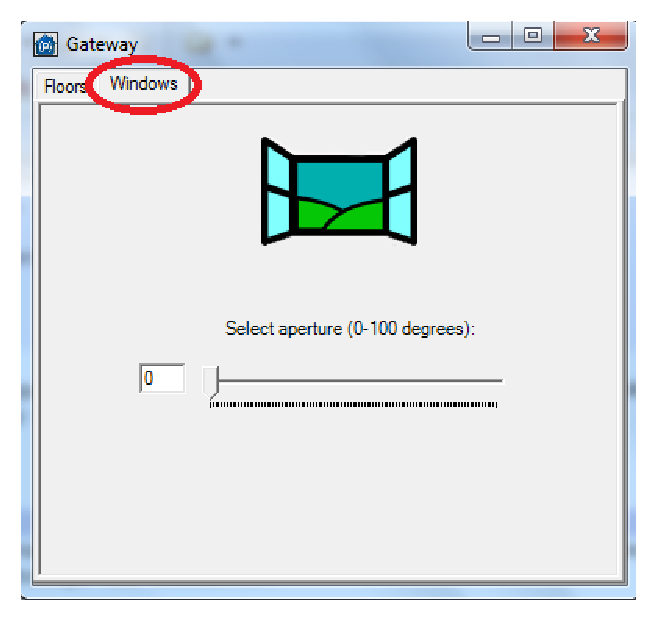
\includegraphics[width=.68\linewidth]{images/globalWindow.eps}
	\\
\vspace{1cm}
\end{center}
\item To change the aperture of the windows, use the slide bar or the text box (press \emph{enter} key to confirm) to introduce a value between 0 to 100.
\end{enumerate}
If you want to change the aperture of a specific window, select the room where is the window, click on the window tab and follow the same steps to modified all windows but in the current tab:
\begin{center}
	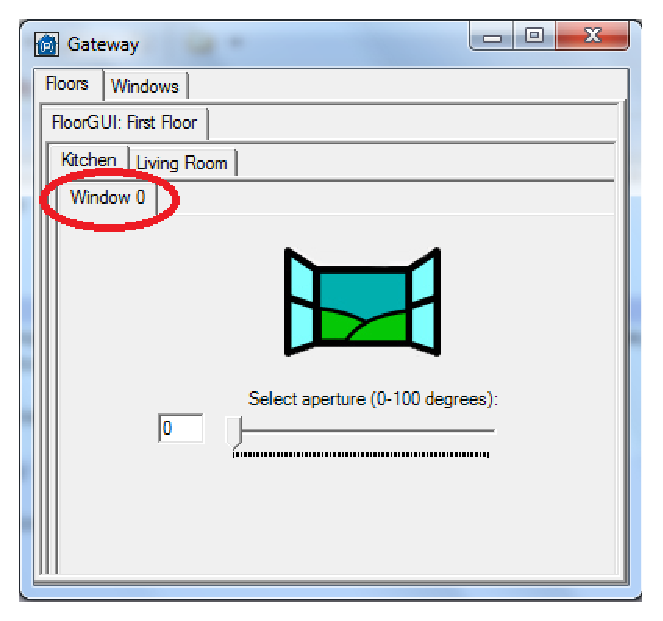
\includegraphics[width=.68\linewidth]{images/specificWindow.eps}
	\\
\vspace{1cm}
\end{center}

In the Simulator window, you have a table with the identifier, room and aperture of each window:
\begin{center}
	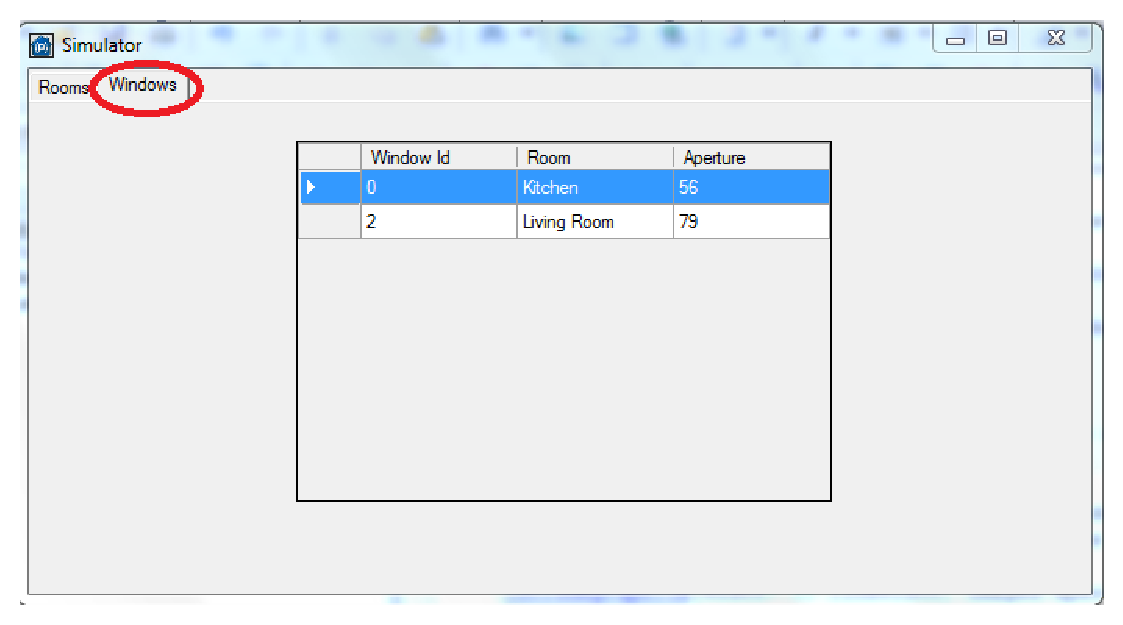
\includegraphics[width=.75\linewidth]{images/simulatorWindow.eps}
	\\
\vspace{1cm}
\end{center}